\chapter{Numerical Semigroups}\label{chap:numsems}

\section{Introduction}\label{sec:smgps:intro}

So far we have only discussed graphs. In this chapter, we will introduce a new object which has a different structure, but for which the Probabilistic Method can be used to prove results. Definitions and results in this chapter can be found in \cite{rosales2009numerical} and \cite{assi2020numerical}. \par

\begin{definition} 
    A \textit{numerical semigroup} is a subset $S \subseteq \NN_{0}$ for which 
    \begin{enumerate}
        \item $0 \in S$,
        \item $S$ is closed under addition, i.e. $a, b \in S$ implies $a + b \in S$, and
        \item $S$ has finite complement in $\NN_{0}$.
    \end{enumerate}
\end{definition}

Examples of numerical semigroups include $\NN_{0}$ and $\NN_{0} \setminus \{1\}$. Subsets of $\NN_0$ which are not numerical semigroups include the set of even numbers, any finite set and $\NN_0 \setminus \{2\}$. Numerical semigroups are studied in the context of commutative algebra and algebraic geometry, and they have applications in coding theory and cryptography \cite{assi2020numerical}. \par

\begin{example}\label{ex:smgps:mcnugget}
    The \textit{McNugget Semigroup} is the set of all non-negative integers which can be expressed as a sum of non-negative multiples of 6, 9 and 20 (see Figure \ref{fig:smgps:mcnugget}).
\end{example}

Suppose you are in the United Kingdom and you wish to order 43 McNuggets. The cashier will hesitate for a while before telling you that they do not sell 43 McNuggets, since there is no combination of boxes of 6, 9 and 20 McNuggets which add up to 43 \cite{youtube}. However, if you order 44 McNuggets, one possibility is that you will receive one box of 20 McNuggets, two boxes of 9 McNuggets and one box of 6 McNuggets. This is because 44 can be expressed as a sum of non-negative multiples of 6, 9 and 20, namely $44 = 2 \cdot 20 + 2 \cdot 9 + 6$. In general, if you order more than 43 McNuggets, you will receive your order. \par

Let us see why the McNugget Semigroup is a numerical semigroup. First, we note that $0$ can be expressed as a sum of non-negative multiples of 6, 9 and 20, namely $0 = 0 \cdot 6 + 0 \cdot 9 + 0 \cdot 20$. Next, we note that if $a$ and $b$ can be expressed as a sum of non-negative multiples of 6, 9 and 20, then so can $a + b$. Finally, we note that the complement of the McNugget Semigroup in $\NN_0$ is finite, since 
\begin{align*}
    44 &= 2 \cdot 20 + 2 \cdot 9 + 6, &45 &= 5 \cdot 9,\\
    46 &= 2 \cdot 20 + 6, &47 &= 20 + 3 \cdot 9,\\
    48 &= 8 \cdot 6, & 49&= 2 \cdot 20 + 9. 
\end{align*}
And every integer greater than 49 can be expressed as a sum of one of these numbers plus a multiple of 6. \par
The McNugget semigroup is an example of a numerical semigroup which is \textit{finitely generated}. This means that there exists a finite set $A = \{a_1, \ldots, a_n\}$ such that $S = \langle A \rangle$, where 
\[\langle A \rangle = \{c_1a_1 + \cdots + c_na_n : c_1, \ldots, c_n \in \NN\}.\]  
\begin{theorem}\label{thm:smgps:fin_gen}
    All numerical semigroups are finitely generated.
\end{theorem}

\textbf{Proof. } Let $S$ be a numerical semigroup. Let $m$ be the first non-zero element of $S$. Let $b_i$ be the first element of $S$ such that \(b_i \equiv i \pmod m\), which exists since $S$ has a finite complement in $\NN$. Let $A = \{m, b_{1}, \ldots, b_{m - 1}\}$. Then $S = \langle A \rangle$, since every non-zero element of $S$ can be expressed as a sum of an element of $A$ plus a non-negative multiple of $m$. \qed \par

Also, note that $\mathrm{gcd}(\{6, 9, 20\}) =  1$.

\begin{theorem}\label{thm:smgps:gcd}
    Let $A \subseteq \NN$ be a non-empty finite set. Then $\langle A \rangle$ is a numerical semigroup if and only if $\mathrm{gcd}(A) = 1$.    
\end{theorem}

\textbf{Proof. } Let $A = \{a_{1} \ldots, a_{n}\}$, where $a_1$ is the first non-zero number in $S = \langle A \rangle$. Note that $a_1$ is in $A$, since it cannot be expressed as the sum of non-negative multiples of other elements in $S$. \par
If $\mathrm{gcd}(A) = d > 1$, then every element in $S$ is divisible by $d$ and so there are infinitely many numbers in $\NN$ which are not in $S$. \par
Now, suppose that $\mathrm{gcd}(A) = 1$. If $a_1 = 1$, then $S = \NN$ is a numerical semigroup. Suppose that $a_1 > 1$. By definition of generating set, $0 \in S$ and S is closed under addtion. Since $\mathrm{gcd}(A) = 1$ then there exist $\lambda_1, \ldots, \lambda_n \in \ZZ$ such that 
\[\lambda_1a_1 + \ldots + \lambda_na_n = 1.\]
Then, 
\[
    k := \sum_{i = 1}^n \lambda_ia_i + a_1\sum_{i = 1}^n|\lambda_i|a_i \equiv 1 \pmod a_1,
\]
and $k$ is a non-negative sum of multiples of elements of $A$: 
\[k = \sum_{i = 1}^n (\lambda_i + |\lambda_i|a_1)a_i,\]
and so $k \in S$. Thus, for $0 \leq j < a_1$, $jk \in S$ and $jk$ is congruent with $j$ modulo $a_1$. Therefore, every number greater than $(a_1 - 1)k$ belongs to $S$, since it can be expressed as the sum of a multiple of $k$ plus a multiple of $a_1$.  This means that the complement of $S$ in $\NN$ is finite and so $S$ is a numerical semigroup. \qed \par

The McNugget semigroup example and the proofs of the previous theorems motivates the following invariants of numerical semigroups. \par 

\section{Invariants}\label{sec:smgps:invariants}

\begin{figure}
    \centering
    %tikz
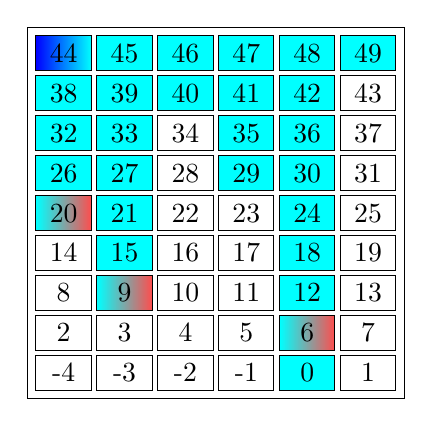
\begin{tikzpicture}[every node/.style={draw,scale=1pt,
    minimum width=20pt,inner sep=3pt,
    line width=0pt,draw=black}]
    \matrix[row sep=2pt,column sep=2pt]
    {\node[left color=blue,right color=-red]{44};&
    \node[fill=-red]{45};&
    \node[fill=-red]{46};&
    \node[fill=-red]{47};&
    \node[fill=-red]{48};&
    \node[fill=-red]{49};\\
    \node[fill=-red]{38};&
    \node[fill=-red]{39};&
    \node[fill=-red]{40};&
    \node[fill=-red]{41};&
    \node[fill=-red]{42};&
    \node[]{43};\\
    \node[fill=-red]{32};&
    \node[fill=-red]{33};&
    \node[]{34};&
    \node[fill=-red]{35};&
    \node[fill=-red]{36};&
    \node[]{37};\\
    \node[fill=-red]{26};&
    \node[fill=-red]{27};&
    \node[]{28};&
    \node[fill=-red]{29};&
    \node[fill=-red]{30};&
    \node[]{31};\\
    \node[left color=-red,right color=red!70]{20};&
    \node[fill=-red]{21};&
    \node[]{22};&
    \node[]{23};&
    \node[fill=-red]{24};&
    \node[]{25};\\
    \node[]{14};&
    \node[fill=-red]{15};&
    \node[]{16};&
    \node[]{17};&
    \node[fill=-red]{18};&
    \node[]{19};\\
    \node[]{8};&
    \node[left color=-red,right color=red!70]{9};&
    \node[]{10};&
    \node[]{11};&
    \node[fill=-red]{12};&
    \node[]{13};\\
    \node[]{2};&
    \node[]{3};&
    \node[]{4};&
    \node[]{5};&
    \node[left color=-red,right color=red!70]{6};&
    \node[]{7};\\
    \node[]{-4};&
    \node[]{-3};&
    \node[]{-2};&
    \node[]{-1};&
    \node[fill=-red]{0};&
    \node[]{1};\\
    };
\end{tikzpicture}
    \caption{Visualization of the McNugget semigroup.}
    \label{fig:smgps:mcnugget}
\end{figure}

Let $S$ be a numerical semigroup. \par

\begin{definition}\label{def:smgps:multiplicity}
    The \textit{multiplicity} of $S$, denoted by $m(S)$, is the smallest non-zero element of $S$.
\end{definition}

For instance, the multiplicity of the McNugget Semigroup is 6. \par

Let $A$ and $B$ be non-empty finite subsets of $\NN$. Then we denote by $A + B$ the set \[\{a + b : a \in A, b \in B\}.\] 

\begin{theorem}\label{thm:smgps:minimal_generating_set}
     There exists a unique minimal generating set $A$ with $S = \langle A \rangle$.
\end{theorem}

\textbf{Proof. } Let $A = S \setminus(S + S)$. This means that every element in $A$ is not the sum of two elements in $S$. First we prove that $A$ generates $S$. Note that $A$ generates 0. Suppose that $s\in S \setminus A$. Then $s = a + b$, such that $a$ and $b$ are in $S$ and $a, b < s$. If we proceed recursively, in a finite number of steps we can express $s$ as a sum of elements of $A$. \par

Now, we show that $A$ is minimal. If $S = \langle A' \rangle$, then for $a \in A$, if $a$ is a sum of non-negative multiples of elements of $A'$, then, since $a$ is not the sum of two elements in $S$, $a$ must be an element of $A'$. \qed \par

Since the minimal generating set is unique, we can define the following invariant.\par

\begin{definition}\label{def:smgps:embedding_dim}
    The \textit{embedding dimension} of $S$, denoted by $e(S)$, is the cardinality of the minimal generating set of $S$.
\end{definition}

\begin{corollary}\label{cor:smgps:embedding_dim}
    $e(S) \leq m(S)$.
\end{corollary}
\textbf{Proof. } Apply Theorem \ref{thm:smgps:minimal_generating_set} and the proof of Theorem \ref{thm:smgps:fin_gen}. \qed \par

Let $n$ be a non-zero element of $S$. \par

\begin{definition}\label{def:smgps:aperyset}
    The \textit{Ap\'ery set} of $n$ in $S$ is the set
\end{definition}
\[\mathrm{Ap}(S, n) = \{s \in S : s - n \notin S\}\]

With the observation that $s - n \notin S$ if and only if $s$ is the first element in its congruence class modulo $n$, the Apéry set can also be defined as  
\[\mathrm{Ap}(S, n) =  \{0, b_1, \ldots, b_{n - 1}\},\]
where $b_i$ is the first element of $S$ such that \(b_i \equiv i \pmod n\). 
For instance, \[\mathrm{Ap}(\langle 6, 9, 20 \rangle, 6) = \{0, 49, 20, 9, 40, 29\}.\]. 
\begin{proposition}
    Each element of $\mathrm{Ap}(S, n)$ is either an element of the minimal generating set or a sum of two elements of $\mathrm{Ap}(S, n)$. 
\end{proposition}
\textbf{Proof. } First, $0 = 0 + 0$. If $0 < s \in \mathrm{Ap}(S, n)$, the other option is that $s = a + b$ such that $a \in S\setminus\mathrm{Ap}(S, n)$ and $b \in S$. But this is not possible, since that means that $a - n \in S$, and so $a - n + b \equiv s \pmod{n}$, which contradicts that $s$ is the first element of its congruence class modulo $n$. \qed \par  
For example, in the case of the McNugget semigroup,
\[29 = 20 + 9, \quad 40 = 20 + 20 \quad \text{and} \quad 49 = 40 + 9.\]
\begin{definition}\label{def:smgps:frobeniusnum}
    The \textit{Frobenius number} of $S$, denoted by $F(S)$, is the largest element of $(\NN \cup \{-1\}) \setminus S$.
\end{definition}

The Frobenius number of the McNugget semigroup is 43. For $n \in S$, using the definition of the Frobenius number, we have that
\begin{equation}\label{eq:smgps:selmer1}
    F(S) = \max (\mathrm{Ap}(S, n)) - n,
\end{equation}
since any number larger than this will belong to $S$. It has been proven that finding the Frobenius number with variable $n$ is an NP-hard problem \cite{ramirez1996complexity}.

\begin{theorem} Let $a, b \in \NN$ such that $\mathrm{gcd}(a, b) = 1$. Then 
    \[F(\langle a, b \rangle) = ab - a - b.\] 
\end{theorem}
\textbf{Proof. } If $a$ and $b$ are relatively prime, then $b$ modulo $a$ generates $\ZZ_a$ and $(a - 1)b$ is the maximum element of $\mathrm{Ap}(\langle a, b\rangle, a)$. Apply equation \ref{eq:smgps:selmer1}. \qed

\begin{definition}
    The \textit{conductor} of $S$, denoted by $c(S)$, is the first element of $S$ greater than $F(S)$, so $c(S) = F(S) + 1$.
\end{definition}
In Figure \ref{fig:smgps:mcnugget}, the elements of the McNugget semigroup are colored with light blue, the elements of the minimal generating set are shown in red and the conductor is shown in dark blue. The lowest element of each column is the first element of its congruence class modulo 6, which is the Apéry set of 6 in the McNugget semigroup. \par

In general, the Apéry set can be used in to calculate many properties of numerical semigroups \cite{apery1946branches}. For instance, it can be used to calculate the cardinality of the set of gaps $G(S) = \NN \setminus S$.

\begin{definition}\label{def:smgps:genus}
    The \textit{genus} of $S$, denoted by $g(S)$, is the cardinality of $G(S)$.
\end{definition}

\begin{proposition} Let $n$ be a non-zero element of $S$. 
    \begin{equation}\label{eq:smgps:selmer2}
        g(S) = \frac{1}{n}\left(\sum_{s \in Ap(S, n)} s\right) - \frac{n - 1}{2}.
    \end{equation}
\end{proposition}
\textbf{Proof. } First, if we divide the complement of $S$ in $\NN$ into congruence classes modulo $n$, we can find the number of gaps in congruence class $i$ by counting the number of elements in that class before the first element of $S$ in that class. Thus, if $b_i \in \mathrm{Ap}(S, n)$ and $b_i \equiv i \pmod n$, we can write $b_i = k_i n + i$, and the number of gaps in congruence class $i$ is $k_i$. Therefore,
\begin{align*}
    g(S) = \sum_{i = 1}^{n - 1} k_i &=  \frac{1}{n}\left(n\sum_{i = 1}^{n - 1} k_i + \frac{n(n - 1)}{2}\right) - \frac{n - 1}{2} \\
    &= \frac{1}{n}\left(\sum_{i = 1}^n k_i n + i \right) - \frac{n - 1}{2} \\
    &= \frac{1}{n}\left(\sum_{s \in Ap(S, n)} s \right) - \frac{n - 1}{2}. \qed
\end{align*}
Equations \ref{eq:smgps:selmer1} and \ref{eq:smgps:selmer2} are known as the \textit{Selmer formulas} \cite{selmer1977linear}. Note that \[g(S) \leq F(S),\] since $F(S)$ is the largest element of $\NN \setminus S$. Also, 
\[g(S) \geq \frac{c(S)}{2} = \frac{F(S) + 1}{2},\]
since $s \in S$ implies that $F(S) - s \notin S$, which means that at least half of the elements which are less than $c(S)$ do not belong to $S$.  This also shows that
\begin{equation}\label{eq:smgps:frobgenus}
    g(S) \leq F(S) \leq 2g(S).
\end{equation}

\section{Wilf's Conjecture}\label{sec:smgps:theme2}

Now, we present a dangerous problem, in the sense that it is easy to state, but it has not been solved yet. Let $n(S)$ be the number of elements of $S$ which are less than $c(S)$, so that $n(S) + g(S) = c(S)$.\par 

\begin{conjecture}[Wilf, 1978] \cite{wilf1978circle}\label{conj:smgps:wilf}
    For any numerical semigroup $S$,
    \[\frac{n(S)}{c(S)} \geq \frac{1}{e(S)}.\]
\end{conjecture}

Wilf's conjecture states that the density of the elements of a numerical semigroup which are less than the conductor (also called the \textit{small elements}) is bounded below by the inverse of the embedding dimension. This conjecture has been verified for specific classes of numerical semigroups \cite{assi2020numerical}: for a numerical semigroup $S$, Wilf's conjecture holds whenever one of these conditions is satisfied:
\begin{itemize}
    \item $e(S) \leq 3$,
    \item $e(S) = m(S)$,
    \item $F(S) - 1 + g(S) \leq 4$,
    \item $4g(S) \leq 3c(S)$,
    \item $n(S) \leq 4$,
    \item $4n(S) \geq c(S)$,
    \item $F(S) \leq 20$.
\end{itemize}

This is not an exhaustive list. As there are several published papers on partial solutions, a recent survey on Wilf's conjecture can be found in \cite{2020conjecture}. \par